%-------------------------------------------------------------------------------------------------------
%-------------------------------------------------------------------------------------------------------
\section{Simulation Analysis}
\label{sec:simulation}


In this section, Circuit T2 is reproduced with the help of Ngspice (each section corresponds
to each task). Ngspice is a simulator for eletronic circuits that can output a variety of results.
This emulator computes the voltages in every node, as well as the potential difference
between two given nodes. Apart from that, the group made use of the command
{\em .options savecurrents} which also enables the output of the currents that pass
through all branches.

With the limitation that Ngspice only provides the current in the components and not through
the nodes, an aditional voltage source ($Vaux$) was added so that the current in $R_6$ ($I_d$)
is known. This source (not displayed in Figure \ref{fig:Dsnh_sim_t2}) has a voltage of 0V and it 
was implemented between $R_6$ and $R_7$. Therefore an aditional node had to be added (node $N7.$).

As previously stated, $I_b$ is refered to as $G_1$. This is because, in Ngspice, a
voltage-controlled current source is identified with capital 'g' ($G$). In the case of
$V_c$, all current-controlled voltage source are identified with $H$.


%-----------------------------------------------------------------------
%-----------------------------------------------------------------------
% 			      task1 - subsec
% ----------------------------------------------------------------------
% ----------------------------------------------------------------------
\subsection{Task 1)}
\label{subsec:task1_s}


In this subsection, the circuit is simulated when $t<0$. There is no need for a
transient analysis because $v_s(t)$=$V_s$ (according to the data given), therefore
all values are constant in time. 

\begin{figure}[ht]
	\centering
	\includegraphics[width=0.75\linewidth]{dsnh_oct_t2_al1.pdf}
	\caption{Circuit T2, analysed by Ngspice}
\label{fig:Dsnh_sim_t2}
\end{figure}

Table \ref{tab:op1} shows the simulated operating point results for Circuit T2.

\begin{table}[ht]
	\centering
	\begin{tabular}{|l|r|}
		\hline    
		{\bf Name} & {\bf Value [A or V]} \\ \hline
    		@cb[i] & 0.000000e+00\\ \hline
@ce[i] & 0.000000e+00\\ \hline
@q1[ib] & 7.022567e-05\\ \hline
@q1[ic] & 1.404513e-02\\ \hline
@q1[ie] & -1.41154e-02\\ \hline
@q1[is] & 5.765392e-12\\ \hline
@rc[i] & 1.411536e-02\\ \hline
@re[i] & 1.411536e-02\\ \hline
@rf[i] & 7.022567e-05\\ \hline
@rs[i] & 0.000000e+00\\ \hline
v(1) & 0.000000e+00\\ \hline
v(2) & 0.000000e+00\\ \hline
base & 2.254108e+00\\ \hline
coll & 5.765392e+00\\ \hline
emit & 1.411536e+00\\ \hline
vcc & 1.000000e+01\\ \hline

	\end{tabular}
	
	\caption{Values from Ngspice. Variables identified with a '$@$' or are of the type
	$i(...)$ have a corresponding value in Ampere (A). The others are expressed in Volts (V).}
    
\label{tab:op1}
\end{table}

The three last entries in Table \ref{tab:op1} provides the potential diference between important
branches: $V_b$ = $v(n5,n2)$ and $V_d$ = $v(n5,n8)$.


%-----------------------------------------------------------------------
%-----------------------------------------------------------------------
% 			      task2 - subsec
% ----------------------------------------------------------------------
% ----------------------------------------------------------------------
\subsection{Task 2)}
\label{subsec:task2_s}


In this subsection, the circuit is simulated when $t=0$. The capacitor is replaced with a voltage source, 
with its value being equal to de diference between the voltages in nodes $n6$ and $n8$ (or $V_x$ = $V(n6)-
V(n8)$) obtained in subsection \ref{subsec:task1_s}. Vs is also set to 0.

This step is necessary to find the boundary conditions of the circuit at $t=0$, which will be used in the next section to calculate the natural response of the T2 circuit.

\begin{figure}[ht]
	\centering
	\includegraphics[width=0.75\linewidth]{dsnh_oct_t2_al2.pdf}
	\caption{Circuit T2, analysed by Ngspice}
\label{fig:Dsnh_sim_t2}
\end{figure}

Table \ref{tab:op2} shows the simulated operating point results for Circuit T2.

\begin{table}[ht]
	\centering
	\begin{tabular}{|l|r|}
		\hline    
		{\bf Name} & {\bf Value [A or V]} \\ \hline
    		i(vaux) & -4.33681e-19\\ \hline
i(h1) & 2.783827e-03\\ \hline
@g1[i] & -2.16736e-18\\ \hline
@r1[i] & -2.06837e-18\\ \hline
@r2[i] & -2.16736e-18\\ \hline
@r3[i] & 9.898797e-20\\ \hline
@r4[i] & 4.379062e-19\\ \hline
@r5[i] & -2.78383e-03\\ \hline
@r6[i] & -4.33681e-19\\ \hline
@r7[i] & 8.858001e-19\\ \hline
n1 & 0.000000e+00\\ \hline
n2 & -2.07580e-15\\ \hline
n3 & -6.50369e-15\\ \hline
n5 & -1.77636e-15\\ \hline
n6 & 8.568097e+00\\ \hline
n7 & 8.729000e-16\\ \hline
n7. & 8.729000e-16\\ \hline
n8 & 1.776357e-15\\ \hline
v(n5,n2) & 2.994417e-16\\ \hline
v(n5,n8) & -3.55271e-15\\ \hline

	\end{tabular}
	
	\caption{Values from Ngspice. Variables identified with a '$@$' or are of the type
	$i(...)$ have a corresponding value in Ampere (A). The others are expressed in Volts (V).}
    
\label{tab:op2}
\end{table}


%-----------------------------------------------------------------------
%-----------------------------------------------------------------------
% 			      task3 - subsec
% ----------------------------------------------------------------------
% ----------------------------------------------------------------------
\subsection{Task 3)}
\label{subsec:task3_s}

In this subsection, the natural response of the circuit was simulated using the boundary conditions
$V(n6)$ and $V(n8)$ calculated in subsection \ref{subsec:task2_s}. Thus, $V_{n6}(t)$ was ploted in the 
interval [0;20]$ms$ (Figure \ref{fig:trans-1}).

\begin{figure}[ht]
	\centering
	\includegraphics[width=0.75\linewidth]{dsnh_oct_t2_al3.pdf}
	\caption{Circuit T2, analysed by Ngspice}
\label{fig:Dsnh_sim_t2}
\end{figure}

\begin{figure}[ht]
	\centering
	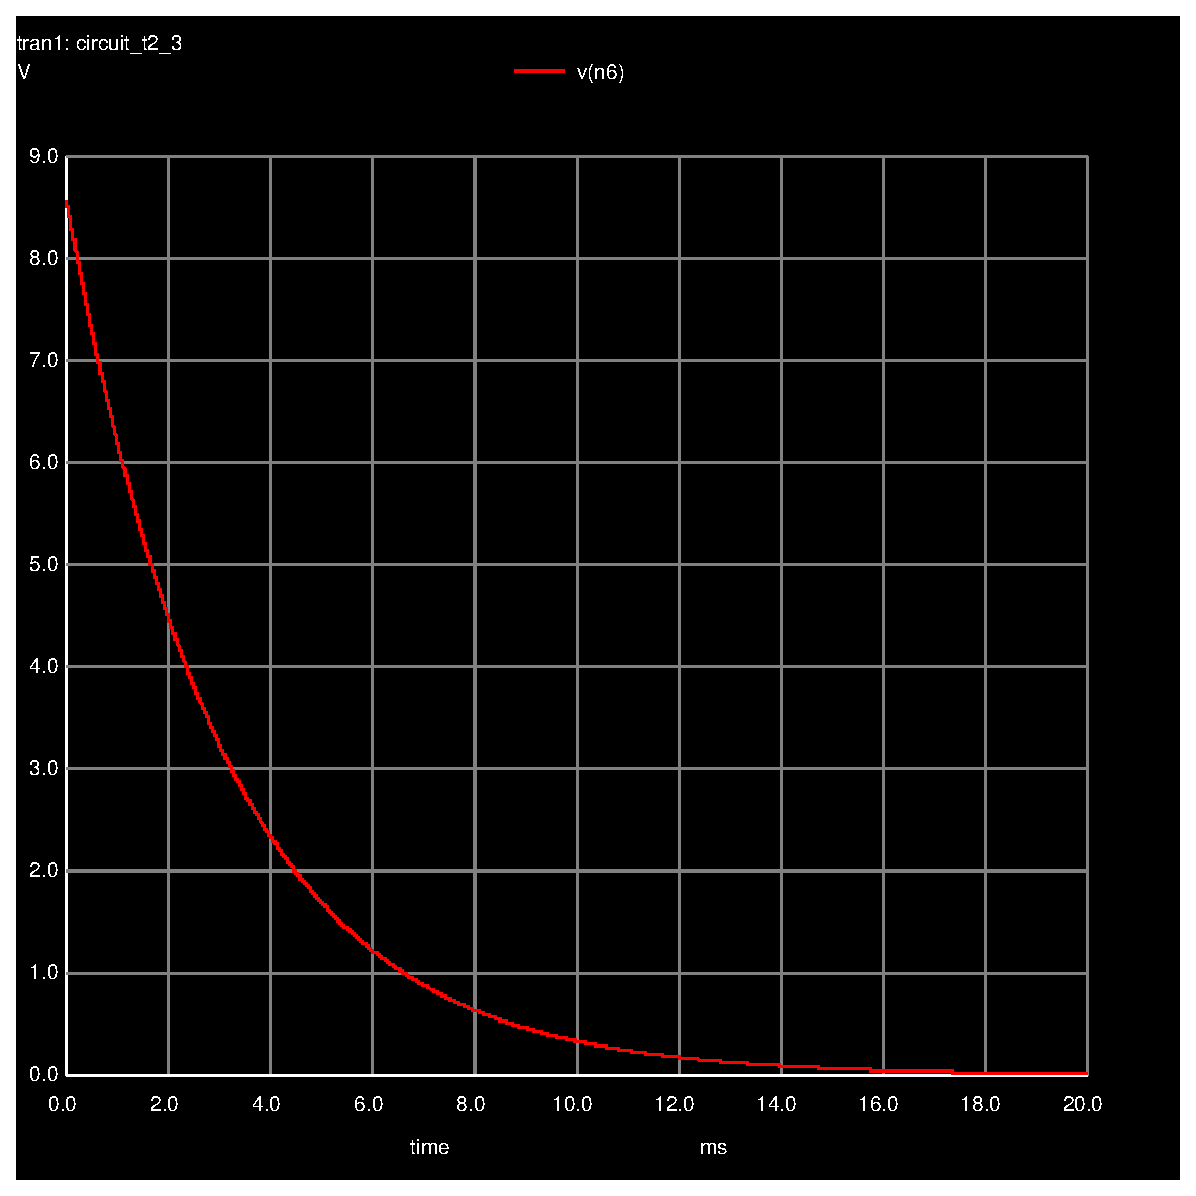
\includegraphics[width=0.55\linewidth]{trans-1.eps}
	\caption{Transient analysis - 1: natural response on node $n6$}
\label{fig:trans-1}
\end{figure}


%-----------------------------------------------------------------------
%-----------------------------------------------------------------------
% 			      task4 - subsec
% ----------------------------------------------------------------------
% ----------------------------------------------------------------------
\subsection{Task 4)}
\label{subsec:task4_s}

In this subsection, the total (natural and forced) responde on node $n6$ is simulated. The boundary
conditions used are the same as subsection \ref{subsec:task3_s} and a frequency of 1kHz (f=1KHz) is
considered for $v_s(t)$. Figure \ref{fig:trans-2} shows the plot. It is worth noting that node $n1$ has
the same value as the stimulus ($v_s(t)$), so $V(n1)$ is used instead.

\begin{figure}[ht]
	\centering
	\includegraphics[width=0.75\linewidth]{dsnh_oct_t2_al456.pdf}
	\caption{Circuit T2, analysed by Ngspice}
\label{fig:Dsnh_sim_t2}
\end{figure}

\begin{figure}[ht]
	\centering
	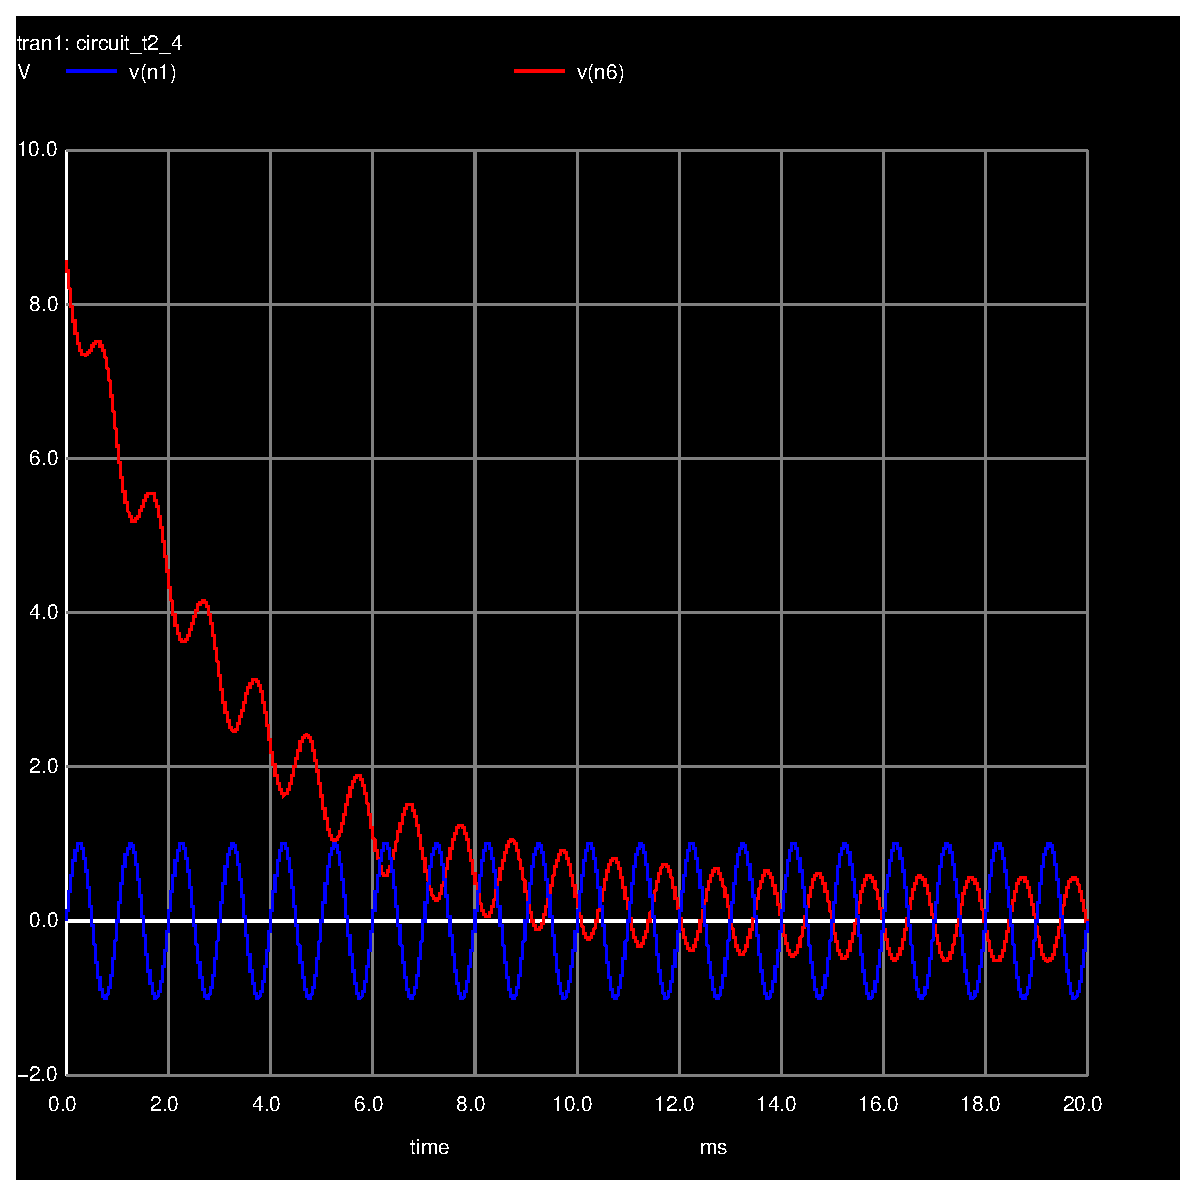
\includegraphics[width=0.55\linewidth]{trans-2.eps}
	\caption{Transient analysis - 2: total response on node $n6$}
\label{fig:trans-2}
\end{figure}


%-----------------------------------------------------------------------
%-----------------------------------------------------------------------
% 			      task5 - subsec
% ----------------------------------------------------------------------
% ----------------------------------------------------------------------
\subsection{Task 5)}
\label{subsec:task5_s}

In this subsection, the frequency response on node $n6$ is simulated.

\begin{figure}[ht]
	\centering
	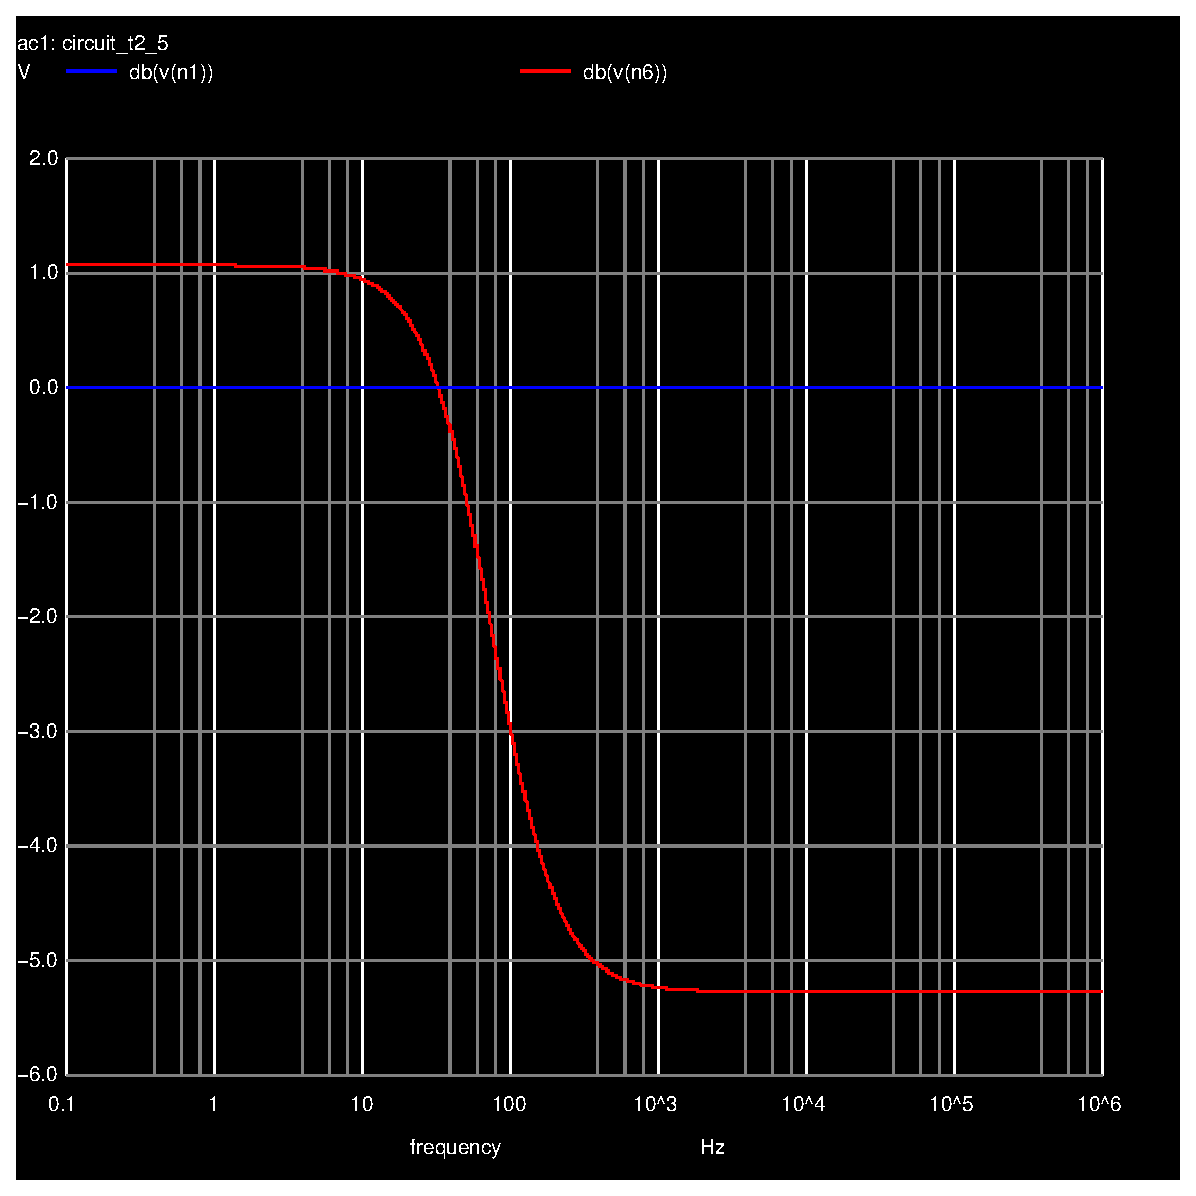
\includegraphics[width=0.55\linewidth]{ac-1.eps}
	\caption{Frequency response - 1}
\label{fig:Dsnh_sim_t2}
\end{figure}

\begin{figure}[ht]
	\centering
	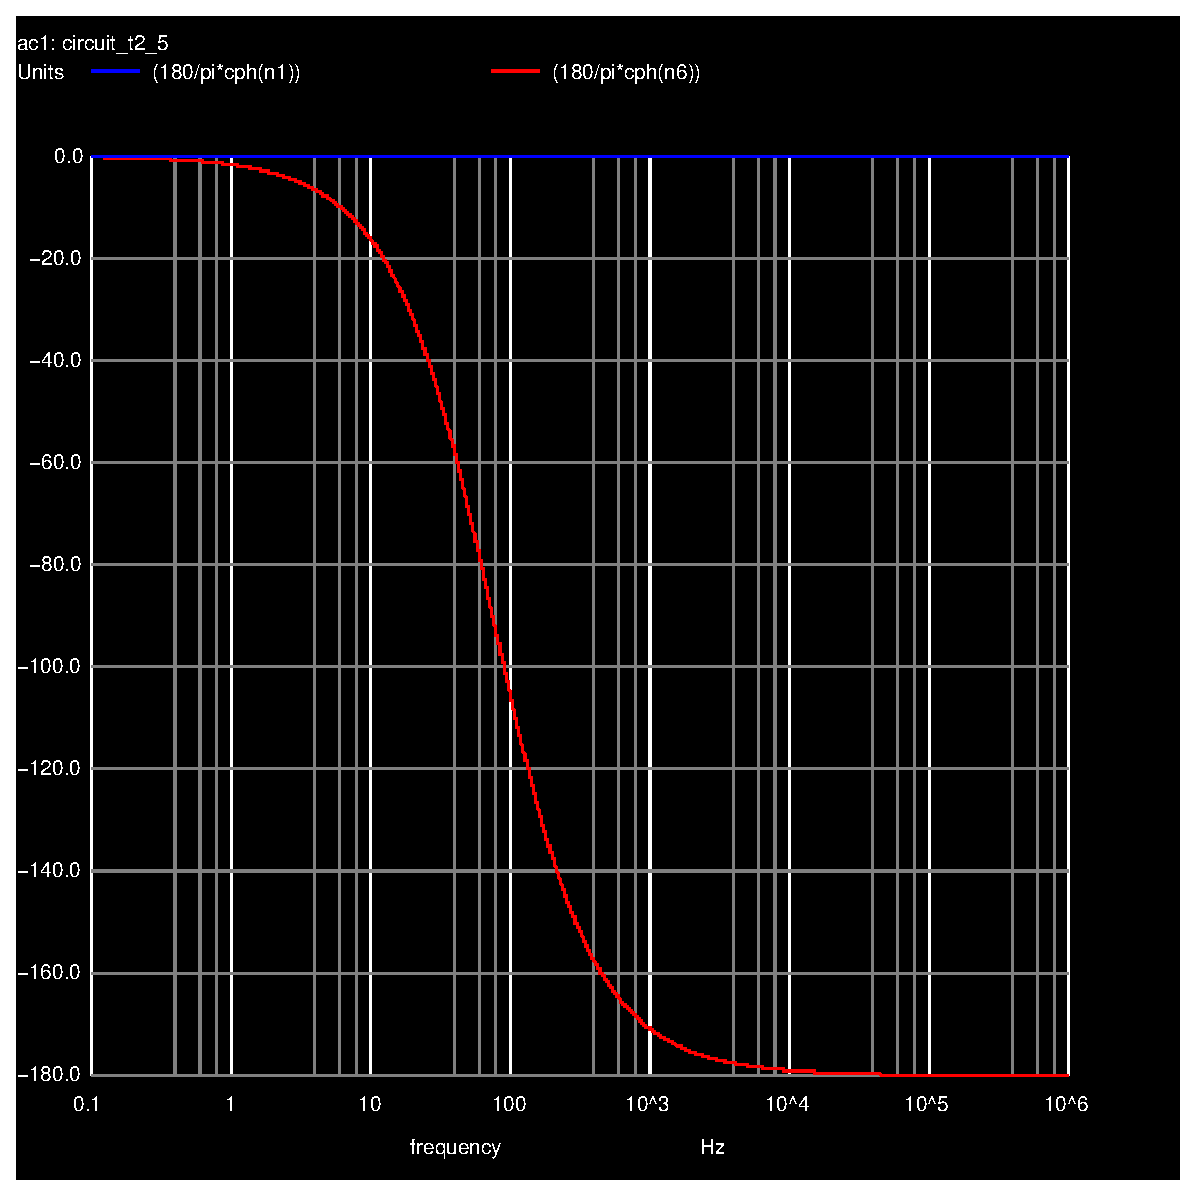
\includegraphics[width=0.55\linewidth]{ac-2.eps}
	\caption{Frequency response - 2}
\label{fig:Dsnh_sim_t2}
\end{figure}


